% Created 2020-07-17 sex 16:02
% Intended LaTeX compiler: pdflatex
\documentclass[11pt]{article}
\usepackage[utf8]{inputenc}
\usepackage[T1]{fontenc}
\usepackage{graphicx}
\usepackage{grffile}
\usepackage{longtable}
\usepackage{wrapfig}
\usepackage{rotating}
\usepackage[normalem]{ulem}
\usepackage{amsmath}
\usepackage{textcomp}
\usepackage{amssymb}
\usepackage{capt-of}
\usepackage{hyperref}
\usepackage{minted}
\usepackage[hyperref, x11names]{xcolor}
\hypersetup{colorlinks = true, urlcolor = SteelBlue4, linkcolor = black}
\usepackage[brazilian]{babel}
\usepackage{geometry}
\geometry{verbose,a4paper,left=2cm,top=2cm,right=3cm,bottom=3cm}
\date{\today}
\title{EP2 Modelagem e Simulação - 2020}
\hypersetup{
 pdfauthor={},
 pdftitle={EP2 Modelagem e Simulação - 2020},
 pdfkeywords={},
 pdfsubject={},
 pdfcreator={Emacs 26.3 (Org mode 9.3.7)}, 
 pdflang={Brazilian}}
\begin{document}

\maketitle
\tableofcontents

\newpage

\section{Introdução}
\label{sec:org35aea3a}
\subsection{Motivação}
\label{sec:orgdf8d0ac}
\paragraph{} Aprender mais sobre simulações de diferentes tipos e 
como elas podem nos ajudar a entender a realidade.
\subsection{Objetivos}
\label{sec:org92aee02}
\paragraph{} Nossos objetivos eram construir dois métodos que simulassem o
desenvolvimento do Corona em diferentes condições.
\section{Materiais e Métodos}
\label{sec:org8712428}
\subsection{Cronograma}
\label{sec:org0c3902b}
\paragraph{} O grupo foi criado no dia 19 de Junho e 
no mesmo dia fizemos uma reunião para 
dividir quem faria qual parte do EP.
Toda a semana a partir dessa data, 
nos reunimos para cada um ver como o 
outro estava se saindo. De modo geral, o progresso atendeu às expectativas do grupo,
embora o volume de trabalho tenha se intensificado perto do fim do projeto.

\begin{itemize}
\item Dia 19 de Junho - Formação do Grupo
\item Dia 20 de Junho - Separação das Tarefas, início das leituras
\item Dia 28 de Junho - Início das pesquisas adicionais, desenho dos módulos a serem programados
\item Dia 4 de Julho  - Finalização do desenho dos módulos, início da programação
\item Dia 12-15 de Julho - Fim da pesquisa. Nessa semana, o grupo se reuniu todos os dias para garantir a finalização do trabalho. Os módulos em jupyter foram finalizados e debugados até o dia 15.
\item Dia 15-17 de Julho - Experimentos e elaboração do relatório. Novamente o grupo se reuniu em todos os dias do período.
\end{itemize}

\begin{figure}[htbp]
\centering
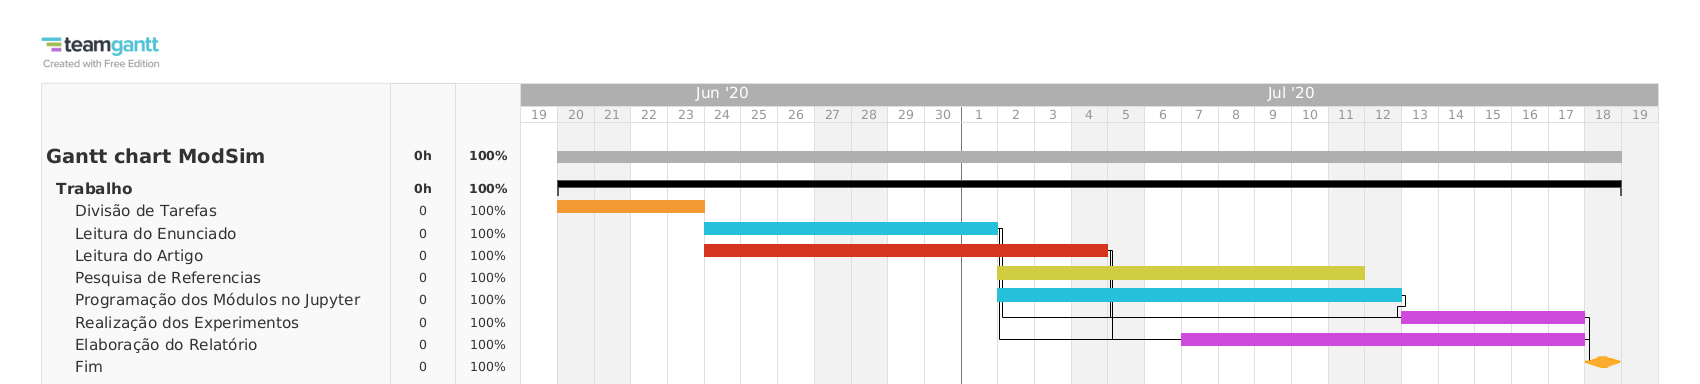
\includegraphics[width=500px]{images/Gantt_chart_ModSim.png}
\caption{Gantt chart do EP, o grupo acredita que o cronograma foi razoavelmente respeitado.}
\end{figure}
\subsection{Ferramentas Utilizadas}
\label{sec:orgea1c91c}
\begin{itemize}
\item Comunicação: Discord
\item Produzir o Código: Jupyter
\item Relatório: Org-mode do Emacs e Overleaf
\end{itemize}
Utilizamos também o artigo do Sonnino para conseguir
dados para usar nos nossos experimentos.
\section{Resultados Experimentais}
\label{sec:org65e25ac}
\subsection{Modelo Dinâmico}
\label{sec:org7ecb80c}
\paragraph{} A primeira coisa que fizemos aqui foi entender
como cada parâmetro alterava o desenvolvimento
da simulação. Fizemos isso para que depois pudéssemos
sortear aleatoriamente os parâmetros para reproduzir
os cenários pedidos no enunciado do EP.

Com esses dados em mãos, começamos a sortear
os parâmetros, tendo como base os valores da Itália e
da Bélgica, já que eram os valores que achamos
no artigo do Sonnino.

Lendo mais um pouco o artigo, descobrimos que o 
\(\lambda\) depende dos parâmetros virais R e \(\mu\) e,
também, do \(t_0\). Como o \(\mu\) é um parâmetro experimental,
não podemos descobrir quanto ele vale, e teremos que
sortear o \(\lambda\).

O caso do \(\alpha\) é diferente, como ele depende do
\(\lambda\) e do \(t_0\) e nós já sorteamos esses valores,
em teoria não podemos sorteá-lo.

Como foi pedido no enunciado que façamos simulações
randomizadas, vamos fazê-las, mas para cada uma,
iremos fazer uma simulação seguindo o artigo.

Com isso em mente, aqui estão algumas das curvas
que conseguimos com este modelo.
\newpage

\subsubsection{Bateria 1 de testes (Seed = Xarabacaia)}
\label{sec:orgcdb014a}
\begin{figure}[htbp]
\centering
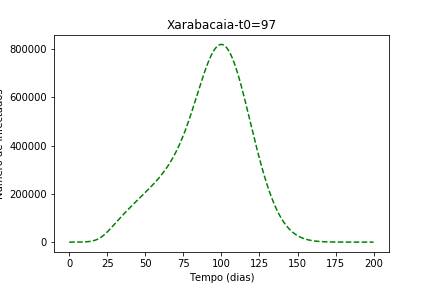
\includegraphics[width=250px]{images/Xarabacaia-t0=97.png}
\caption{Simulação com o dia 97 como início da quarentena e o resto dos parâmetros completamente randômicos. Podemos perceber que como a quarentena começa após quase 100 dias do começo do surto, a curva tem um pico muito alto e fino, indicando que muitas pessoas se infectaram simultaneamente.}
\end{figure}

\begin{figure}[htbp]
\centering
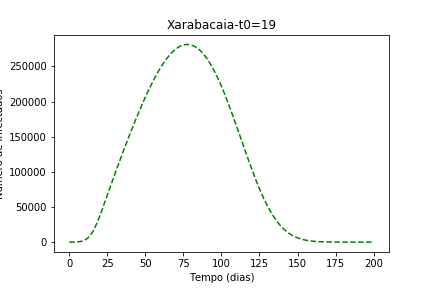
\includegraphics[width=250px]{images/Xarabacaia-t0=19.png}
\caption{Simulação com o dia 19 como início da quarentena e o resto dos parâmetros iguais aos da imagem anterior. Aqui, percebemos que a curva tem um pico menor (31,25\%) e é mais achatada que a da simulação anterior, indicando que a quarentena conseguiu, eficientemente, reduzir o contagio da doença.}
\end{figure}

\begin{figure}[htbp]
\centering
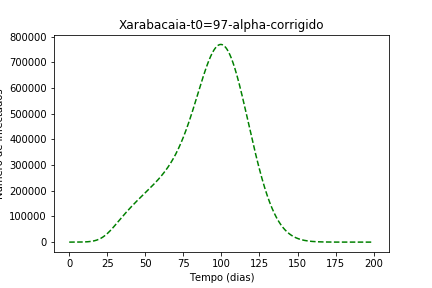
\includegraphics[width=250px]{images/Xarabacaia-t0=97-alpha-corrigido.png}
\caption{Esse gráfico é o mesmo da imagem 1, só que com o \(\alpha\) corrigido. Podemos perceber que a diferença nesse caso não é tão grande.}
\end{figure}

\begin{figure}[htbp]
\centering
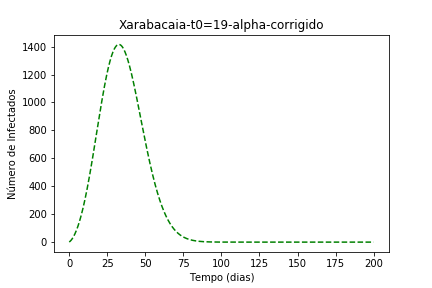
\includegraphics[width=250px]{images/Xarabacaia-t0=19-alpha-corrigido.png}
\caption{Gráfico da imagem 2 com o \(\alpha\) corrigido. Aqui se torna evidente a diferença que o \(\alpha\) corrigido faz, o pico ficou mais do que 100 vezes menor, mostrando a verdadeira eficiência da quarentena.}
\end{figure}
\newpage
\subsubsection{Bateria 2 de testes (Seed = cknorris)}
\label{sec:org5d2b7ac}
\begin{figure}[htbp]
\centering
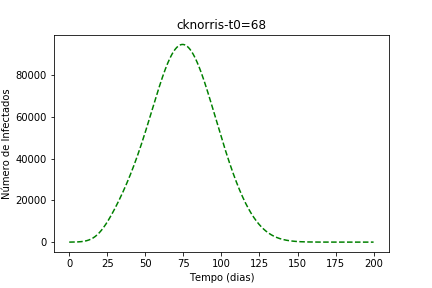
\includegraphics[width=250px]{images/cknorris-t0=68.png}
\caption{Simulação com o início da quarentena no dia 68 e o resto dos parâmetros randomizados. Podemos perceber as semelhanças com o gráfico respectivo do item anterior, só que com a escala 10 vezes menor.}
\end{figure}

\begin{figure}[htbp]
\centering
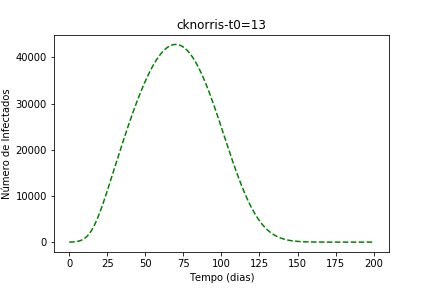
\includegraphics[width=250px]{images/cknorris-t0=13.png}
\caption{Simulação com o início da quarentena no dia 13 e o resto dos parâmetros iguais aos da imagem anterior. Podemos ver que a quarentena diminuiu pela metade o tamanho do pico e o deixou uma pouco mais achatado, como esperado.}
\end{figure}

\begin{figure}[htbp]
\centering
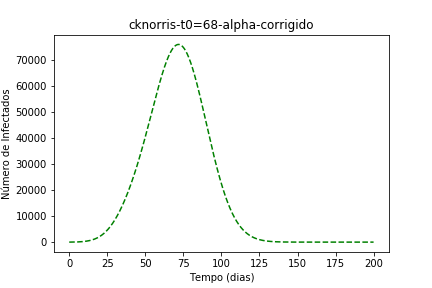
\includegraphics[width=250px]{images/cknorris-t0=68-alpha-corrigido.png}
\caption{Gráfico da imagem 5 com o \(\alpha\) corrigido. Podemos perceber, apenas, que a correção do \(\alpha\) diminuiu um pouco o pico do gráfico.}
\end{figure}

\begin{figure}[htbp]
\centering
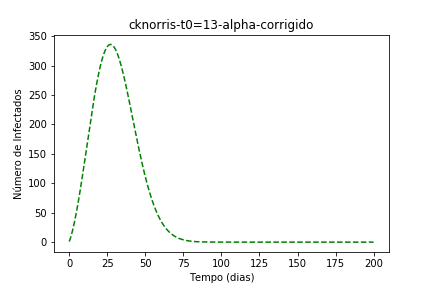
\includegraphics[width=250px]{images/cknorris-t0=13-alpha-corrigido.png}
\caption{Gráfico da imagem 6 com o \(\alpha\) corrigido. Podemos ver aqui o mesmo efeito que aconteceu na bateria de testes anterior. Ao corrigir o \(\alpha\) percebemos a verdadeira eficiência da quarentena, diminuindo em mais de 10 vezes o tamanho do pico.}
\end{figure}
\newpage    
\subsubsection{5 ilhas}
\label{sec:org7324990}
\begin{figure}[htbp]
\centering
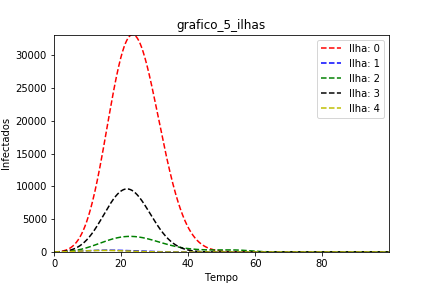
\includegraphics[width=250px]{images/grafico_5_ilhas.png}
\caption{Imagem feita ao simular o método dinâmico para 5 ilhas diferentes, com parâmetros diferentes.}
\end{figure}

\begin{figure}[htbp]
\centering
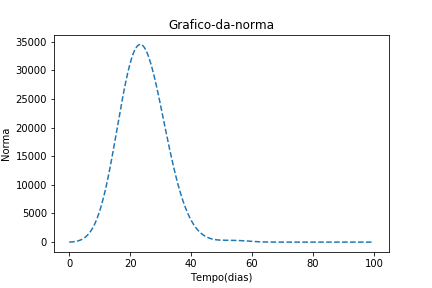
\includegraphics[width=250px]{images/Grafico-da-norma.png}
\caption{Gráfico feito a partir da norma do vetor das 5 ihas que estão representadas na imagen anterior.}
\end{figure}

\subsection{Modelo Estocástico}
\label{sec:org9f195dc}
\paragraph{} Esse modelo têm uma quantidade bem maior de
parâmetros, o que fez com que tivéssemos muita
liberdade para simular várias situações diferentes.
Levamos em conta desde de condições sociais como
tamanho da família e número de aglomerações por dia, 
até parâmetros virais como probabilidade de infecção
por encontro, tempo de incubação e período infeccioso.

Fizemos também um sistema de quarentena, que caso
ativado, fará com que alguém infectado tenha uma
certa chance de entrar em quarentena a cada dia,
fazendo com que essa pessoa fique em casa até
ser curada.

O objetivo principal dessa simulação era verificar
afirmações de que a imunidade de manada (mínimo 
de pessoas infectadas por COVID-19) suficiente para
impedir a transmissão do coronavírus seria em torno de
20\%. Para tanto, criamos um modelo aleatório que gera
uma população de pessoas que tem uma certa quantidade
de outras pessoas dentro de uma série de clusters,
de tal modo que uma pessoa tem muito mais chance de 
encontrar alguem que está dentro de um dos seus clusters.

Uma vez que os clusters são gerados, um dos indivíduos na população
é infectado e a cada dia um numero de encontros é processado para cada
pessoa. Quando uma pessoa infectada encontra uma não infectada, há
uma chance de passar a infecção. Ao longo do tempo, pessoas podem morrer,
se curar e ficar imunes (e portanto impossíveis de ser infectadas)
ou podem entrar em quarentena(representando tanto isolamento doméstico quanto doentes graves que são recolhidos ao hospital), e portanto param de encontrar outras pessoas.
O modelo "clusterizado" é de interesse porque, se quaisquer duas pessoas
tiverem a mesma chance de se encontrar, estamos fazendo um modelo muito distante
da realidade, uma vez que a chance de alguém encontrar uma pessoa que mora no
mesmo domicílio, por exemplo, é muito maior do que a chance de encontrar
uma pessoa que vive do outro lado da cidade.

O modelo também contabiliza o fator de multiplicação do vírus R de modo que possamos
verificar se os parâmetros geram uma taxa de replicação viral que tem correspondência com
os valores observados na realidade.

Sobre a imunidade de manada, o modelo obtem valores máximos em torno de 98\% e valores mínimos muito
baixos, para parâmetros que mantém o maior valor de R observado entre 1 e 6 (de acordo com os valores
estimados para o COVID-19 na literatura.\(^{[1]}\)

Abaixo relacionamos as curvas de infectados no tempo para uma série de parâmetros, com a mesma
semente. Os \texttt{.csv} têm como nome a semente utilizada, seguida de um número que corresponde ao gráfico.
Para os experimentos abaixo, foi usada a semente "XARABACAIA". Em todos, variamos apenas a chance de quarentena, o tamanho dos clusters, a infectividade do virus e o numero de encontros que cada pessoa pode ter por dia. Outros parâmetros como a duração da doença, o tempo de incubação do virus e o tempo de incubação necessário para infectar outros ficaram constantes.

\begin{figure}[htbp]
\centering
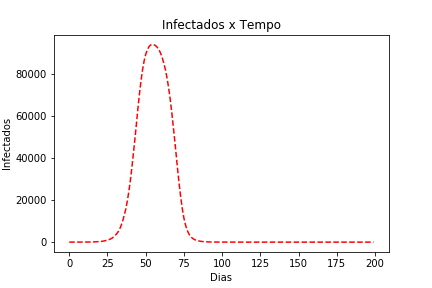
\includegraphics[width=250px]{images/XARABACAIA1.png}
\caption{Figura padrão de uma epidemia descontrolada. Quase toda a população foi infectada, gerando imunidade de manada 98,5\%. Os clusters e a quantidade de encontros por dia eram altos(100 e 30), e a chance de quarentena baixa. 2000 pessoas morreram, de 100.000. Valor R máximo: 10 Arquivo: XARABACAIA1.csv}
\end{figure}
\begin{figure}[htbp]
\centering
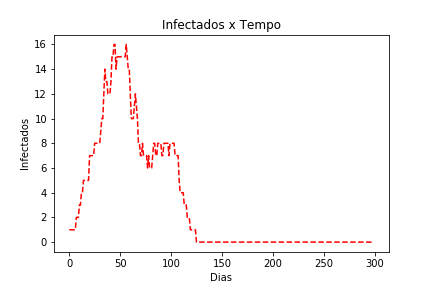
\includegraphics[width=250px]{images/XARABACAIA2.png}
\caption{Figura de uma epidemia totalmente controlada. De 100.000 pessoas, 37 foram infectadas. Não houve mortes. Nesse caso, os clusters e a quantidade de encontros por dia eram ambos menores, e a chance de quarentena mais alta. A imunidade de manada certamente não foi atingida. Valor R máximo: 1,2 Arquivo: XARABACAIA2.csv}
\end{figure}
\begin{figure}[htbp]
\centering
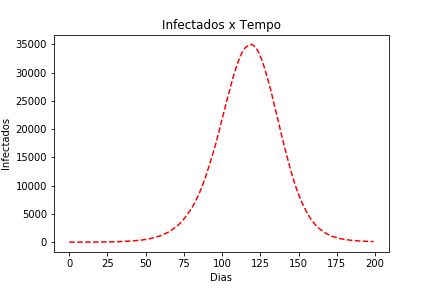
\includegraphics[width=250px]{images/XARABACAIA6.png}
\caption{Figura de uma epidemia mal controlada. A imunidade de manada ficou em 65,8\%, e houve 1354 mortes. Os clusters eram do mesmo tamanho da figura 1, mas a chance de quarentena era maior, e a infectividade do virus e numero de encontros menores. Valor R máximo: 2. Arquivo: XARABACAIA6.csv}
\end{figure}
\begin{figure}[htbp]
\centering
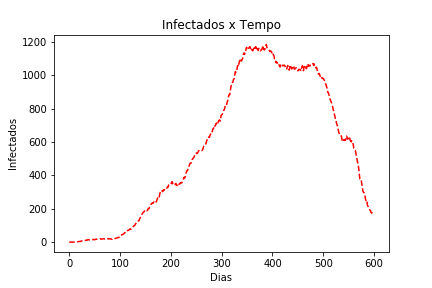
\includegraphics[width=250px]{images/XARABACAIA9.png}
\caption{Figura de uma epidemia em "estado estável": Há mais de 100 dias no gráfico em que o número de infectados se mantém  quase constante. Nesse caso, a infectividade do virus era intermediária, mas o número de encontros baixo e chance de quarentena alta. Houve 282 mortes e a imunidade de manada ficou em torno de 12,8\% Valor R máximo: 1.2. Arquivo: XARABACAIA9.csv}
\end{figure}

\newpage
\section{Conclusão}
\label{sec:org90c942f}
\subsection{Modelo Dinâmico}
\label{sec:orgef795bc}
\paragraph{} Primeira coisa que podemos concluir é como cada parâmetro influencia o desenvolvimento da doença:

\begin{itemize}
\item \(\alpha\): Taxa de Crescimento viral, quanto maior
mais rápido o vírus irá espalhar.
\item A: Algo relacionado à permissividade do meio ao
corona. Quanto maior, mais rápido o vírus irá
espalhar
\item \(t_0\): Início da quarentena. Quanto menor,
menos o virus espalha e mais achatada a curva fica.
\item \(\lambda\): Fator que relaciona a transmissividade
do vírus com a sua taxa de reprodução. Quanto maior,
mais rápido o vírus se espalha.
\end{itemize}

Outra coisa que percebemos com os nossos experimentos é que ao usar o alpha corrigido, 
a quarentena fica muito mais eficaz.
Isso se deve ao fato de que o \(\alpha\) depende do \(t_0\) e do \(\lambda\), então nas simulações que os três eram decididos 
aleatoriamente, conseguíamos resultados inconsistentes.

Já que os únicos parâmetros verdadeiramente livres que temos são o A e o \(t_0\), podemos concluir também que segundo
esse modelo, a evolução da pandemia é completamente controlável caso a quaretenta seja respeitada.
\subsection{Modelo Estocásticco}
\label{sec:orgd325498}
\paragraph{} É interessante notar que o principal fator que determina se uma infecção será controlada ou não é efetivamente a diminuição do contato entre as pessoas, seja diminuindo o número de encontros, seja aumentando a chance de quarentena entre as pessoas. A infectividade do vírus, isto é, a chance de que um dado encontro gere uma infecção, é um fator importante, além de outros que podemos citar, como o período de duração da infectividade, e a duração total da doença. Contudo, não se verificou a esperança de que em um quadro de infecção descontrolada, isto é, absoluta ausência de políticas publicas de isolamento, com o único tipo de quarentena sendo a remoção ao hospital(de modo que a chance de quarentena está em 20\%, aproximadamente a chance de casos graves de COVID-19), a imunidade de manada chegaria num patamar em torno de 70\% e isso causaria o fim da transmissão.

Com efeito, não se observa um tal impedimento da transmissão até que quase a totalidade das pessoas esteja infectada nesse caso. Os experimentos que apresentaram imunidades de manada baixa o fizeram porque esses modelos também tinham chances altas de quarentena e pouco encontro entre as pessoas.

A esperança de que clusters pequenos e alta restrição de pessoas aos seus clusters impediriam a propagação do corona (uma vez que todo um cluster fosse infectado a infecção pararia de ser transmitida) se revelaram infundadas, pela alta conectividade entre os clusters. Esse resultado era esperado, considerando por exemplo um resultado famoso de ciencias sociais em que a distância social entre dois indíviduos quaisquer pode ser tão pouco quanto 3 indivíduos\(^{[2]}\). Mesmo com parâmetros baixos de infectividade do vírus, uma tal interconexão social entre os clusters leva a um quadro de transmissão violenta e disseminada. Portanto, mesmo um vírus pouco infeccioso pode alcançar parcela significativa da população.

Nossos resultados reforçam, então, que para um vírus com fator reprodutivo como o do COVID-19, entre 1 e 6 em média, o isolamento social é altamente efetivo para conter o avanço da epidemia e, crucialmente, evitar um número elevado de mortes.
\newpage
\section{Contribuição dos Autores}
\label{sec:org17e6ed7}
\paragraph{} Nome, NUSP e contribuição de cada um.\\

Lourenço Henrique Moinheiro Martins Sborz Bogo - 11208005
\begin{itemize}
\item Relatório
\item Método Dinâmico
\item Auxílio no Método Estocástico
\item Leitura e compreensão do artigo do Sonnino
\item Pesquisa de parâmetros sobre o COVID-19\\
\end{itemize}

Miguel de Mello Carpi - 11208502
\begin{itemize}
\item Animações
\item CSV
\item Auxílio no Método Estocástico
\item Auxílio no Método Dinâmico
\item Leitura e compreensão do artigo do Sonnino\\
\end{itemize}

Eduardo Brancher Urenha - 8587409
\begin{itemize}
\item Relatório
\item Método Estocástico
\item Auxílio no Método Dinâmico
\item Leitura e compreensão do artigo do Sonnino
\item Pesquisa de parâmetros sobre o COVID-19
\item Gantt Chart
\end{itemize}
\section{Referências}
\label{sec:org819cf86}
\begin{enumerate}
\item Liu et al, The reproductive number of COVID-19 is higher compared to SARS coronavirus. Journal of Travel Medicine, Volume 27, Issue 2, March 2020, taaa021. \url{https://doi.org/10.1093/jtm/taaa021}. Published: 13 de Fevereiro, 2020
\item Edunov et al. Three and a half degrees of separation. \url{https://research.fb.com/?s=edunov}. 4 de Fevereiro, 2015. Epub
\item Sonnino e Nardone, Dynamics of the COVID-19 -- Comparison between the Theoretical Predictions and Real Data, 30 Março, 2020. arXiv:2003.13540 [q-bio.PE]. Epub.
\end{enumerate}
\end{document}